\section{Evolutionary Analysis}

\begin{figure}
% \begin{minipage}{6in}
\begin{center}

\begin{minipage}{0.05\textwidth}
~
\end{minipage}%
\begin{minipage}{0.95\textwidth}
\begin{minipage}{0.05\textwidth}
~
\end{minipage}%
\begin{minipage}{0.95\textwidth}
\centering
\large
\textbf{Mean Degree}
\end{minipage}
\begin{minipage}{0.05\textwidth}
~
\end{minipage}%
\begin{minipage}{0.95\linewidth}
\begin{minipage}{0.5\textwidth}
\centering
\large
1
\end{minipage}%
\begin{minipage}{0.5\textwidth}
\centering
\large
2
\end{minipage}
\end{minipage}
\end{minipage}\\
\vspace{2ex}





\begin{minipage}{0.05\textwidth}
\large
\rotatebox[origin=c]{90}{\textbf{Structure}}
\end{minipage}%
\begin{minipage}{0.95\textwidth}
\begin{minipage}{0.05\linewidth}
\large
\rotatebox[origin=c]{90}{Irregular}
\end{minipage}%
\begin{minipage}{0.95\linewidth}
\begin{subfigure}[b]{0.5\textwidth}
\centering
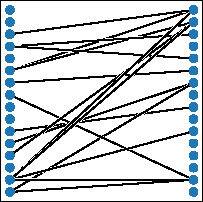
\includegraphics[width=\textwidth]{img/graph_layouts/title=irregular-1+ext=}%
\caption{
Irregular w/ mean degree 1
}
\label{fig:irregular_1}
\end{subfigure}
\begin{subfigure}[b]{0.5\textwidth}
\centering
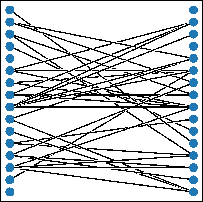
\includegraphics[width=\textwidth]{img/graph_layouts/title=irregular-2+ext=}%
\caption{
Irregular w/ mean degree 2
}
\label{fig:irregular_2}
\label{fig:irregular_degree_2}
\end{subfigure}

\end{minipage}

\vspace{2ex}

\begin{minipage}{\textwidth}

\begin{minipage}{0.05\linewidth}
\large
\rotatebox[origin=c]{90}{Regular}
\end{minipage}%
\begin{minipage}{0.95\linewidth}
\begin{subfigure}[b]{0.5\textwidth}
\centering
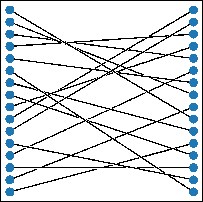
\includegraphics[width=\textwidth]{img/graph_layouts/title=regular-1+ext=}%
\caption{
Regular w/ mean degree 1
}
\label{fig:regular_degree_1}
\label{fig:regular_1}
\end{subfigure}
\begin{subfigure}[b]{0.5\textwidth}
\centering
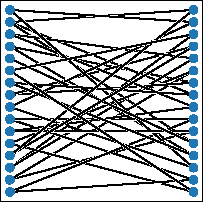
\includegraphics[width=\textwidth]{img/graph_layouts/title=regular-2+ext=}%
\caption{
Regular w/ mean degree 2
}
\label{fig:regular_degree_2}
\label{fig:regular_2}
\end{subfigure}
\end{minipage}
\end{minipage}
\end{minipage}

\caption{
Example target graph layouts used in 32-node graph-matching evolutionary experiments.
Blue dots represent tagged nodes.
Black lines represent selected-for tight affinity relationships.
Layouts differ in total number of selected-for affinities (``mean degree'') and whether selected-for affinities were evenly or randomly distributed between nodes (``structure'').
}
\label{fig:graph_layouts}


\end{center}
% \end{minipage}
\end{figure}


fitness function was based on rank matching.
Randomly generated bipartite graph as a target.
Degree, which refers to the mean number of edges attached to each node.
Regular edges were generated by randomly connecting the bipartite graph such that all left nodes and all right nodes had the same number of connections.
Irregular edges were generated by randomly adding left to right connections.
In this case, some left nodes may have more than the mean degree of edges and some left nodes may have no or fewer than the mean degree of edges.
Likewise for right nodes.
Figure \ref{fig:graph_layouts} depicts these graph layouts.

Genomes consisted of bitstring tags, sixteen representing left nodes in the bipartite graph and sixteen representing right nodes.
To evaluate the fitness of a genome, we harvested the right node tags and placed them in a tag-matching data structure that returns the ranked ordering of tag matches for a particular query tag.
Then, queried the tag-matching data structure with each left node tag in the genome.
We cut down the ranked ordering list returned to the number of the left node tag's outgoing connections in the bipartite target graph.
Fitness was calculated as the fraction of these remaining right node results that corresponded to edges in the bipartite target graph.

We performed 512-generation evolutionary runs with population size 500 and tournament size 7.
We tested combinations of two target graph types: irregular/regular edge layout and mean degree 1 or mean degree 2.
For each configuration, we surveyed each metric's performance over ten per-bit mutation rates ranging from 0.75 expected mutations per genome to 16.0 expected mutation rates per genome.
(Supplementary Figure \ref{fig:evolve_mutsweep} summarizes these results, confirming that each metric/target graph configuration shows a local maximum of performance within the range of mutation rates surveyed.)
For each metric and target graph configuration combination, we chose the most favorable mutation rate defined by sum population-maximum fitness across updates.
We ran 100 replicate evolutionary runs for each mutation rate/target graph/metric combination.

\begin{minipage}{\linewidth}
\begin{center}

\begin{minipage}{\linewidth}
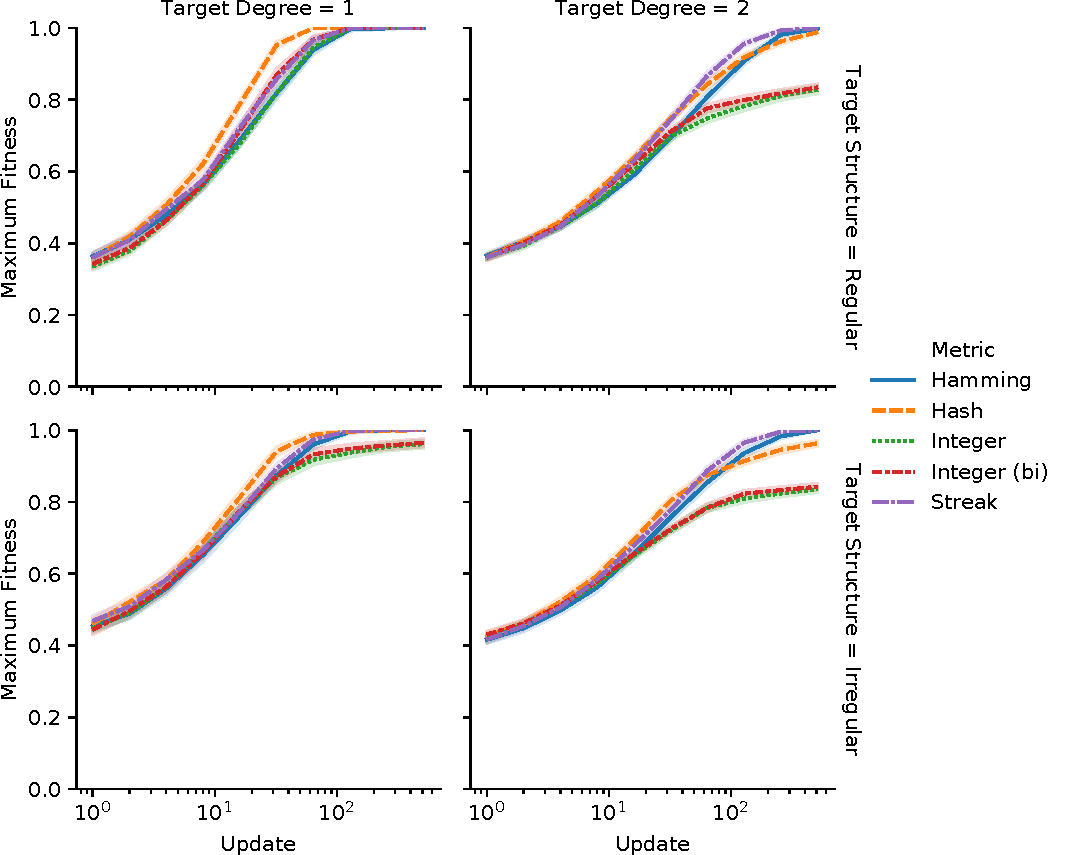
\includegraphics[width=\linewidth]{target_evolve/viz=max-fitness-line+_data_hathash_hash=673d309ab90e91d1+_script_fullcat_hash=fe3ddc711c5abfad+ext=}
\end{minipage}
\begin{minipage}{\linewidth}
\caption{
Maximum fitness by update over replicate runs for each metric's best-performing mutation rate.
Note log-scale x-axes.
Shaded area represents 95\% confidence intervals.
}
\label{fig:evolve_bests}
\end{minipage}
\end{center}
\end{minipage}


Figure \ref{fig:evolve_bests} plots population-maximum fitness across evolutionary runs.
Unsurprisingly, the hash metric performs much more poorly than all other metrics (non-overlapping 95\% confidence intervals).
The integer metrics are capable of evolving solutions to the one-to-one matching problem of the mean degree 1, regular target graph.
However, on mean degree 2 target graphs they evolve significantly poorer quality solutions.

The streak metric performs favorably or equivalently compared to all other metrics across all target graph configurations.
The streak metric yields significantly more rapid adaptive evolution than all other metrics on the regular mean degree 2 graph (non-overlapping 95\% CI).


